\documentclass[25pt,a1paper]{tikzposter}
\geometry{paperwidth=350cm,paperheight=185cm} % or 340 x 150 cm, 500x200
\geometry{left=20cm, right=20cm, top=27cm, bottom=5cm}

% To use an OpenType font with your LaTeX document: 
\usepackage{fontspec, pdfpages}
\setmainfont{DFZongKaiHK-W7.otf}  % USD500 on 2023/06/12
%\setmainfont[[ExternalLocation=/usr/share/fonts/]]{DFZongKaiHK-W7.otf}


%% Tikzposter is highly customizable: please see
%% https://bitbucket.org/surmann/tikzposter/downloads/styleguide.pdf
% x keeping on page one => baposter (http://www.brian-amberg.de/uni/poster/

\tikzposterlatexaffectionproofoff
\let\clearpage\relax

\usepackage{caption}
%\captionsetup{labelformat=empty,listformat=empty}

% clash :-)
%\usepackage[left=20mm, right=20mm, top=30mm, bottom=20mm]{geometry}
%\geometry{left=20cm, right=20cm, top=5cm, bottom=5cm}


% setting tikzposter; deafault {60}{72}
%\settitle{\centering{\@titlegraphic \par \bfseries \fontsize{70}{82} \sc  \@title \par}}

\usepackage{svg, xcolor}
%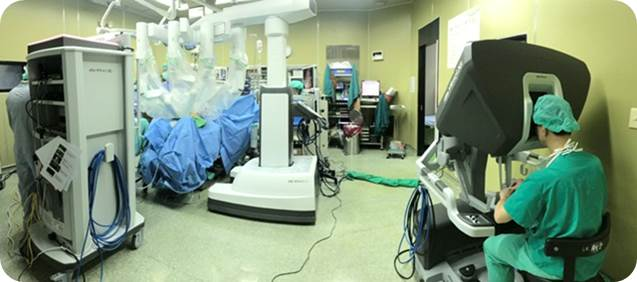
\includegraphics{TMWH_daVinci.jpg}

% a guide: https://roboticsconference.org/information/sample-poster2.pdf
% http://ctan.mirrors.hoobly.com/graphics/pgf/contrib/tikzposter/tikzposter.pdf
%% Available themes: see also
%% https://bitbucket.org/surmann/tikzposter/downloads/themes.pdf
% \usetheme{Default}
% \usetheme{Rays}
% \usetheme{Basic}
 \usetheme{Simple}
%\usetheme{Envelope}
% \usetheme{Wave}
% \usetheme{Board}
% \usetheme{Autumn}
% \usetheme{Desert}

%% Further changes to the title etc is possible
% \usetitlestyle{Default}
% \usetitlestyle{Basic}
% \usetitlestyle{Empty}
% \usetitlestyle{Filled}
% \usetitlestyle{Envelope}
% \usetitlestyle{Wave}
% \usetitlestyle{verticalShading}

\usepackage{fontspec}
\setmainfont{FreeSerif}
\setsansfont{FreeSans}

\usepackage{anyfontsize}
 % Commands
 \newcommand{\bs}{\textbackslash}   % backslash
 \newcommand{\cmd}[1]{{\bf \color{red}#1}}   % highlights command


%    https://tex.stackexchange.com/questions/499066/how-to-increase-the-font-size-of-the-body-in-tikzposter

% https://taipeimedicaltourism.org/en/facility/detail/43

%\title{HANDOVER CEREMONY OF TRAUMA KITS FROM TAIWAN REPRESENTATIVE OFFICE FOR MINISTRY OF HEALTH DEVELOPMENT}

%{TAIWAN MEDICAL MISSION IN THE REPUBLIC OF SOMALILAND}
%\author{With electric operating tables, surgeons can easily adjust the height, lateral tilt, Trendelenburg, and reverse Trendelenburg of the table with the press of a button.}
%\institute{Taiwan Medical Mission in the Republic of Somaliland}
%% Optional title graphic

%\titlegraphic{
%\includesvg[width=0.5\linewidth]{ROC_flag.svg}
%\hspace{3cm}
%\includesvg[width=0.17\linewidth]{TMM_logo.svg}
%\hspace{3cm}
%\includesvg[width=0.5\linewidth]{Somaliland_flag.svg}
%}

% Taipei_5f994223a0add.jpg 
% https://www.mastersportal.com/search/master/medicine-health/taiwan
% 24cm
%% Uncomment to switch off tikzposter footer
% \tikzposterlatexaffectionproofoff

\begin{document}


%%%
%\maketitle

%%%%%%%
\begin{center} % to remove Fig.

\begin{tikzfigure}[]

%\captionsetup{labelformat=empty}
%Taiwan\\
%\vspace{5cm}
\includesvg[height=30.0cm, distort=false]{Flag_of_the_Republic_of_China.svg} \hspace{20cm}
%\includesvg[height=40.0cm]{Blood_logo.svg}\hspace{20cm} % Heart_hands_logo.png
%\hspace{3cm}
\includesvg[height=30.0cm, distort=false]{Flag_of_Somaliland.svg}
\vspace{5cm}
\end{tikzfigure}
\end{center}



%%% title; font size and baseline offset (line space)
\fontsize{260}{300} \sc
%\textcolor{red}{badbaadada hooyaday, waa in ay mudaadiiba mar heshaa shaybaadh} \\ %Maalinta dhiig shubista aduunka} \\ World Blood Donor Day
%2023-10-17 
Save LIVES For World Trauma Day \\
- Bone Health Kick-off and \\
 Handover Ceremony \\
%Campaign\\


%Muwaadin fadlan ugu deeq dhiigaaga walalahaaga u baahan \\
%GIVE BLOOD, GIVE PLASMA, SHARE LIFE, SHARE OFTEN \\

\fontsize{260}{300} \sc
%shaybaadhista  kanserka ilmo galeenka
%Cervical Cancer Screening Program \\
A Multi-Specialty Conference 
\includegraphics[width=0.08\textwidth]{QRcode_2023MSC.png}


%\fontsize{230}{300} \sc %{260}{280}
%\textcolor{red}{Saving My Mother, One Screening at a Time}\\ 

\fontsize{220}{300} \sc
Taipei Municipal Wanfang Hospital \textcolor{red}{versus} Hargeisa Group Hospital\\
On \textcolor{red}{October 17}, 2023, at 09:00 am, Tuesday \\
Venue: Conference Hall of Carro Edeg Hotel, Hargeisa

%Cervical Cancer Screening Since 2023 July \\
%FOR MINISTRY OF HEALTH DEVELOPMENT AND \\
%MINISTRY OF EMPLOYMENT, SOCIAL AFFAIRS AND FAMILY\par
% World Blood Donor Day, WBDD 2023/06/14
%Give blood, give plasma, share life, share often
\vspace{7cm}

%%%%%%%%%%%% from portrait agenda
%%% title; font size and baseline offset (line space)
%\fontsize{20}{24} \sc
%2023 Collaborating for Better Health: \\
%A Multi-Specialty Conference \\
%on Taiwan and Somaliland
% \par
%\vspace{0.3cm}
% FOR MINISTRY OF HEALTH DEVELOPMENT

%\fontsize{12}{13} \sc
%Taipei Municipal Wanfang Hospital versus Hargeisa Group Hospital\\
%On August 13-14, 2023, at 09:00 am, Sunday-Monday \\
%Venue: Conference Hall of Carro Edeg Hotel, Hargeisa
%Exhibition Hall of the Hargeisa Group Hospital
% no more Jees Hotel
%\par
%\vspace{0.2cm}

%%%%%%%%%%%

%%% footer
%\block{}{
%\node [above right,
%       outer sep=0pt,
%       minimum width=\paperwidth-2*\pgflinewidth,
%       minimum height=7cm,
%       align=center,font=\Huge,
%       draw,fill=green!30,
%       ultra thick] at ([shift={(0.5*\pgflinewidth,0.5*\pgflinewidth)}]bottomleft) 
%       {

\begin{tikzfigure}[]
%\includesvg[height=40.0cm, distort=false]{ortho_ward_Tex_Josh.svg}
\includesvg[height=20.0cm]{TRO_Somaliland_font_ZongKai.svg} \hspace{10cm} % object converted to path in Inkscape; TRO_Somaliland_font_ZongKai.eps
% TMWH_logo_TAIPEI_vector; TMWH_logo(noWord)
\includesvg[height=20.0cm, distort=false]{TMWH_logo_TAIPEI_vector.svg}\hspace{10cm}
%\includesvg[height=25.0cm]{anti_CervicalCancer_logo.svg}\hspace{10cm} % Heart_hands_logo.png
\includesvg[height=20.0cm, distort=false]{TMM_logo.svg}\hspace{10cm}
%\includesvg[height=25.0cm, distort=false]{Muslim_women_1.svg}\hspace{10cm} % anti-cervical cancer
%\includesvg[height=20.0cm, distort=false]{Hargeisa_Group_Hospital_logo.svg}\hspace{10cm}
\includesvg[height=20.0cm, distort=false]{logo_MoHD_HGH.svg}
%{MoHD_Somaliland.svg}
%\hspace{1cm} % https://mohd.govsomaliland.org/
%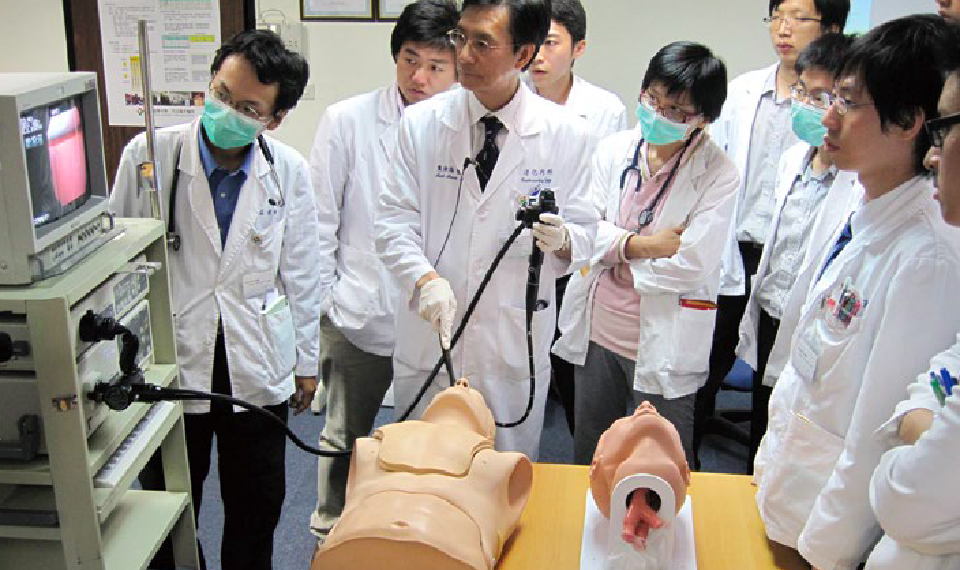
\includegraphics{TMWH_scope.pdf}

%
\includegraphics[height=21.0cm]{TMWH_logo_TAIPEI_vector.pdf}
%\includesvg[height=25.0cm, distort=false]{TMWH_logo.svg}\hspace{1cm} % TMWH with TAIPEI
%\includesvg[height=23.0cm, distort=false]{TMM_logo.svg}
%
\includegraphics[height=24cm]{Puhsein_fundation_TW.png}
%{2023TMM_officePlate_pink.svg}
%\includesvg[height=23.0cm, distort=false]{Hargeisa_Group_Hospital_logo.svg}
%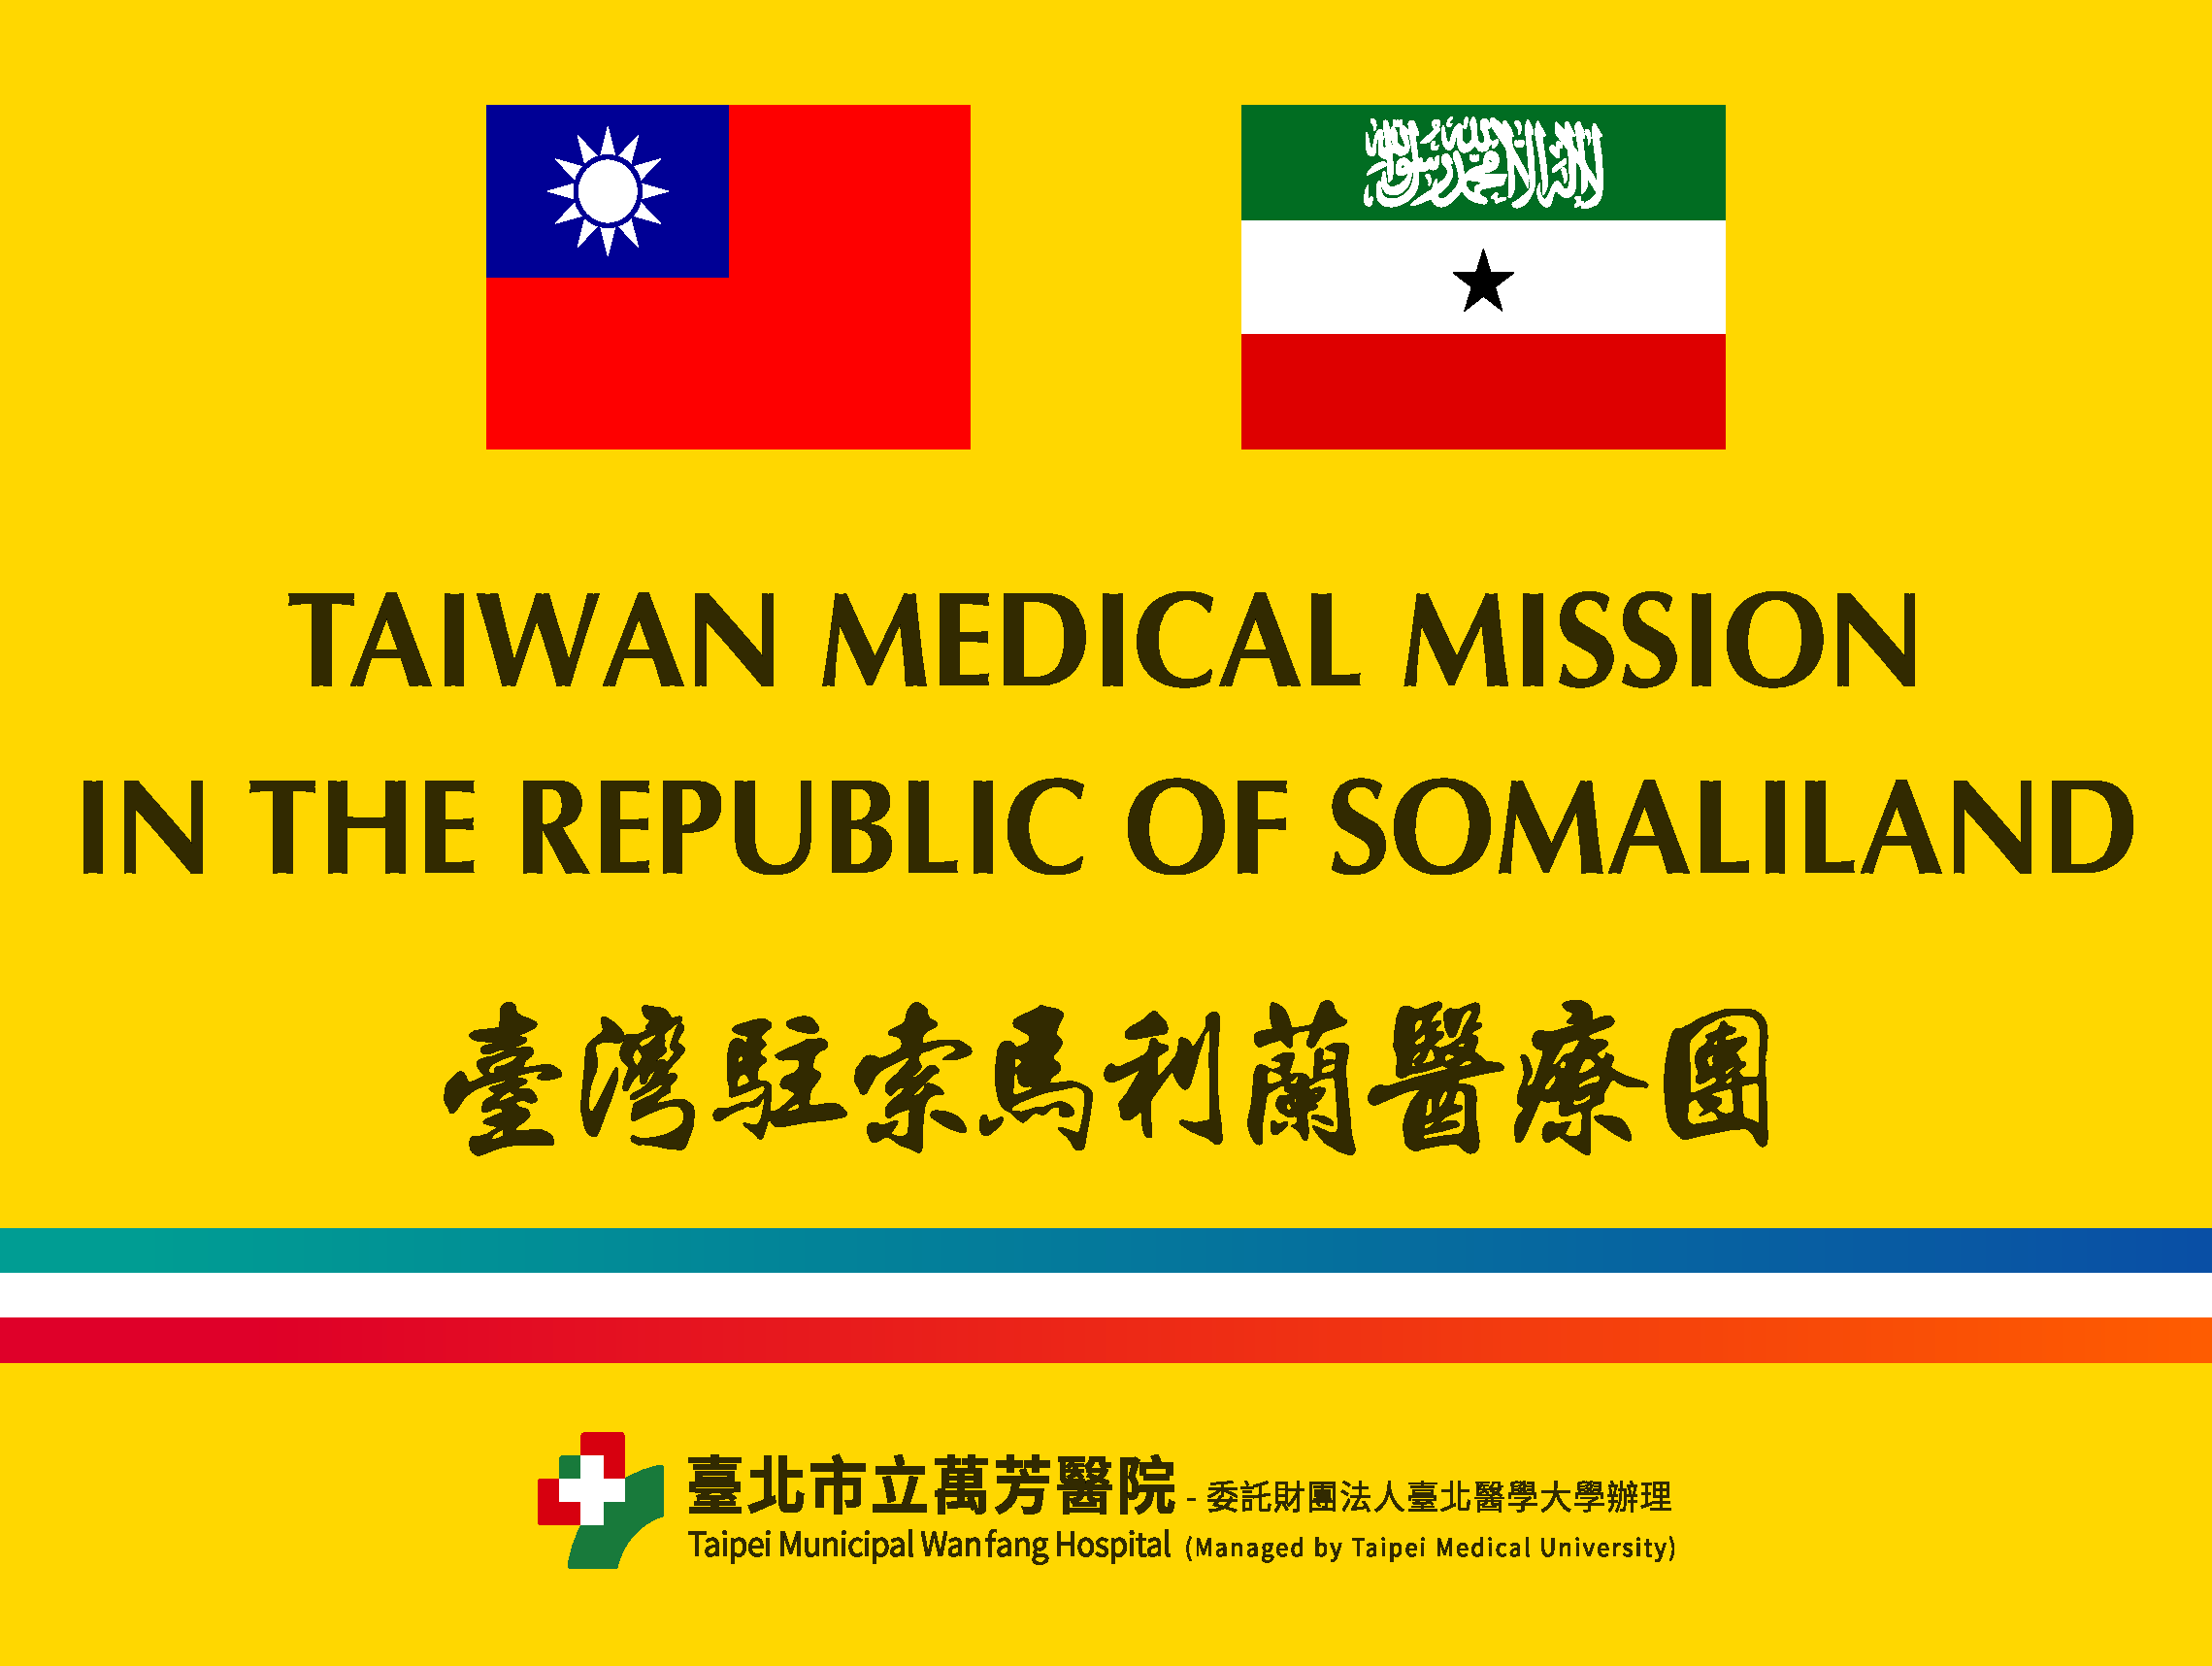
\includegraphics[height=12.0cm, distort=false]{2023TMM_officePlate_ai.pdf}

%%% *********
% ?? add logo of military and social welfare ??



\end{tikzfigure}

%}; % end of node

%} % end of block

\end{document}



%%%%%%%% spared TMU hospitals
% Figures of TMU
\begin{minipage}{0.45\linewidth}
  \centering %456
    \begin{tikzfigure}[]
    % TMWH
    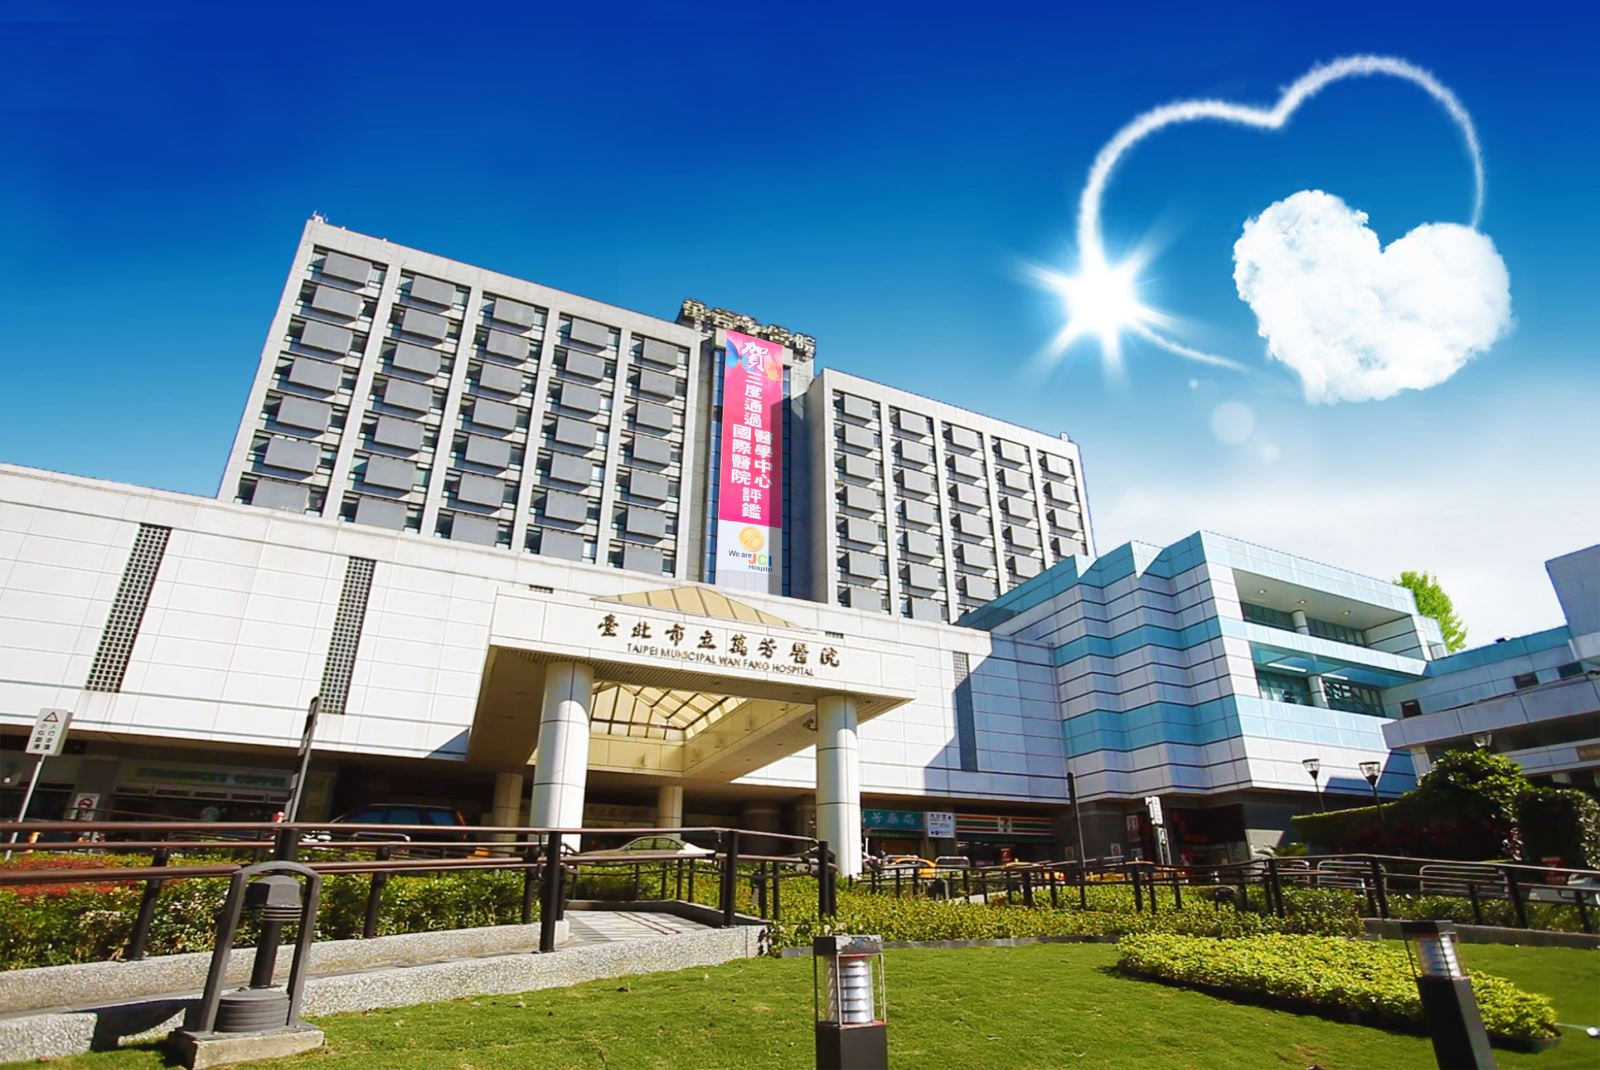
\includegraphics[width=0.7\linewidth]{5FAB9DAB-B258-4FC5-AED2-BB8F415E616F.jpeg}
    % TMUH
    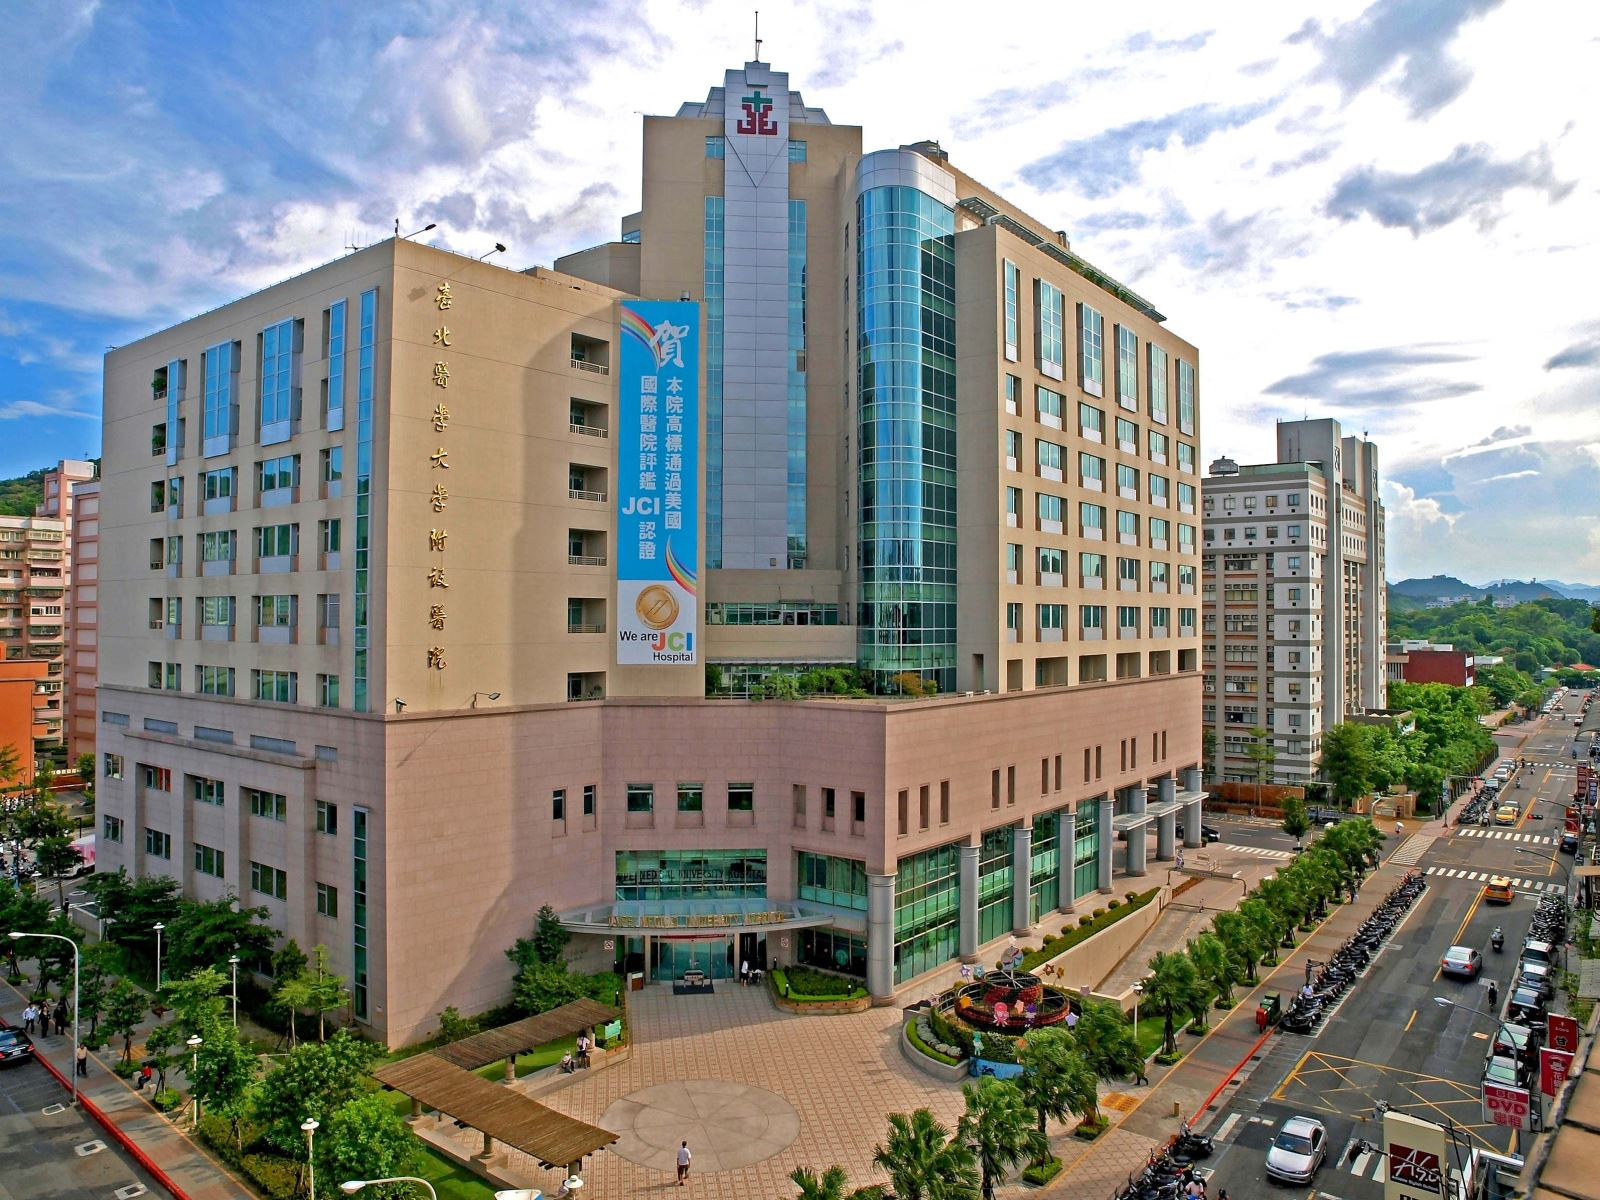
\includegraphics[width=0.7\linewidth]{5782F8B7-D58E-4601-A26D-18DFB462B6B8.jpeg}
    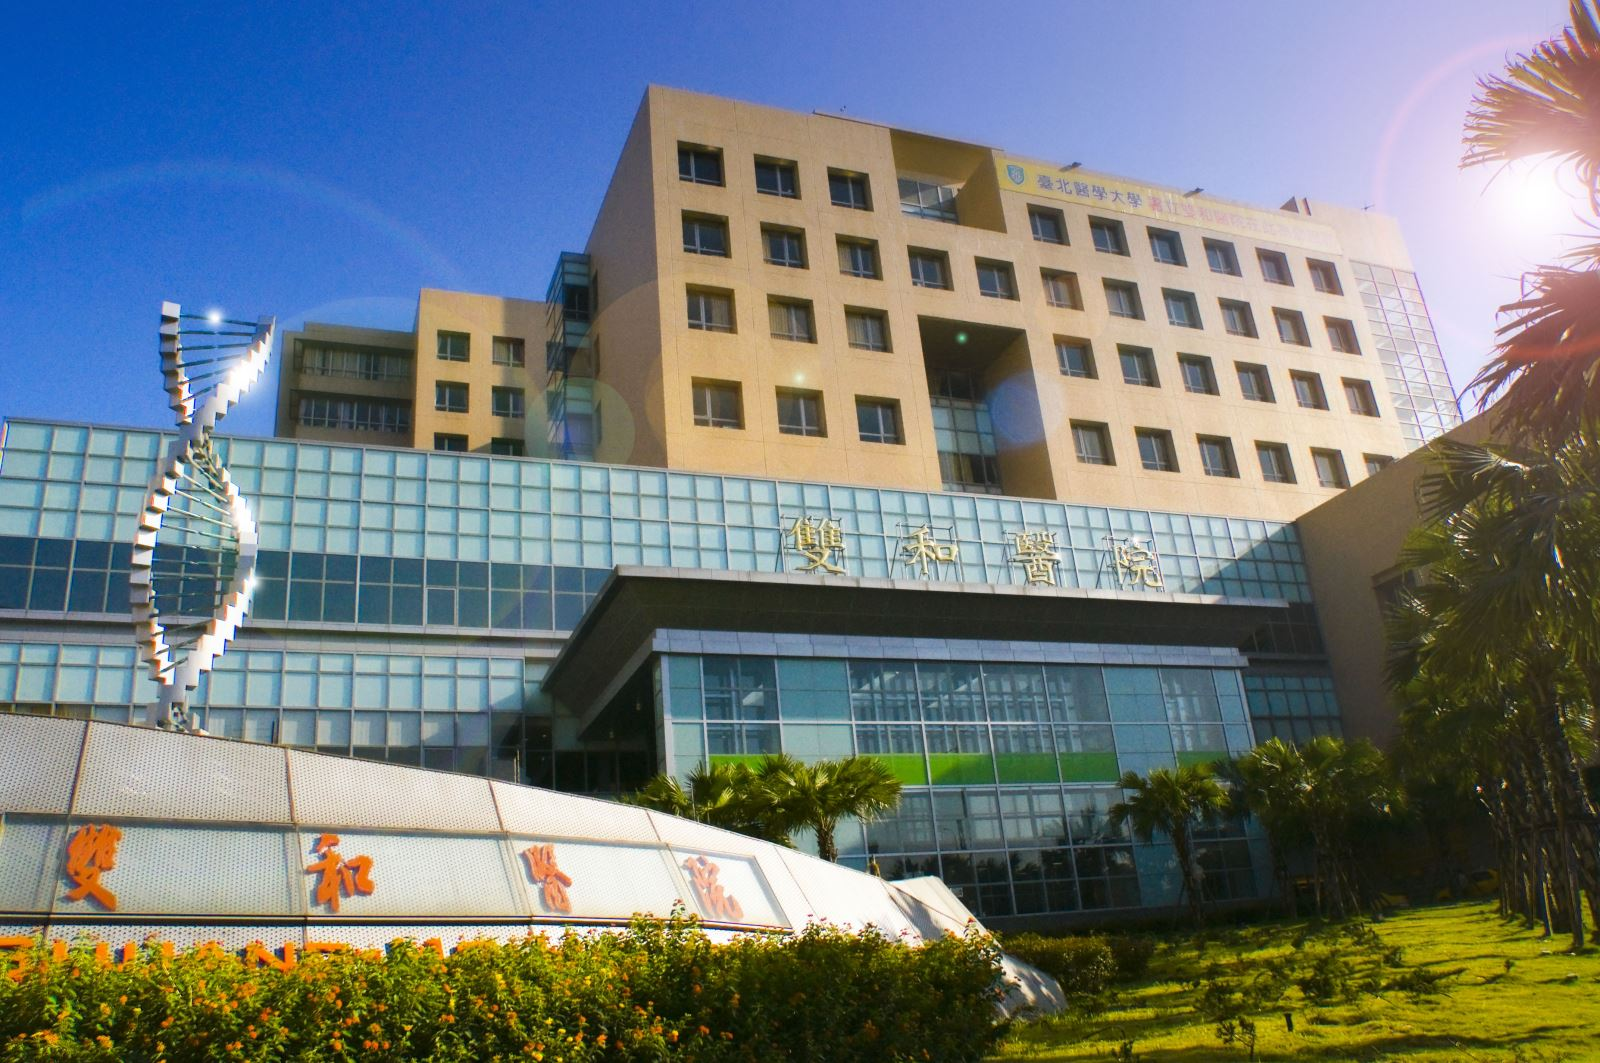
\includegraphics[width=0.7\linewidth]{10885B17-3876-4B24-B689-4B1ACDB21AB3.jpeg}
    \end{tikzfigure}
\end{minipage}\hfill
\begin{minipage}{0.45\linewidth}
  \centering
%\innerblock{TMU's Hospitals}{
    \begin{tikzfigure}[]
    %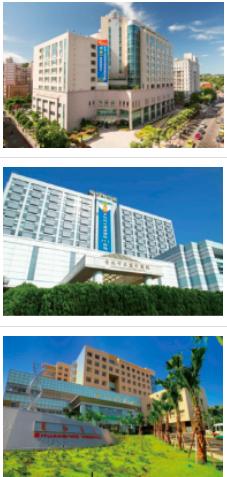
\includegraphics[width=0.5\linewidth]{TMU123.jpg}
    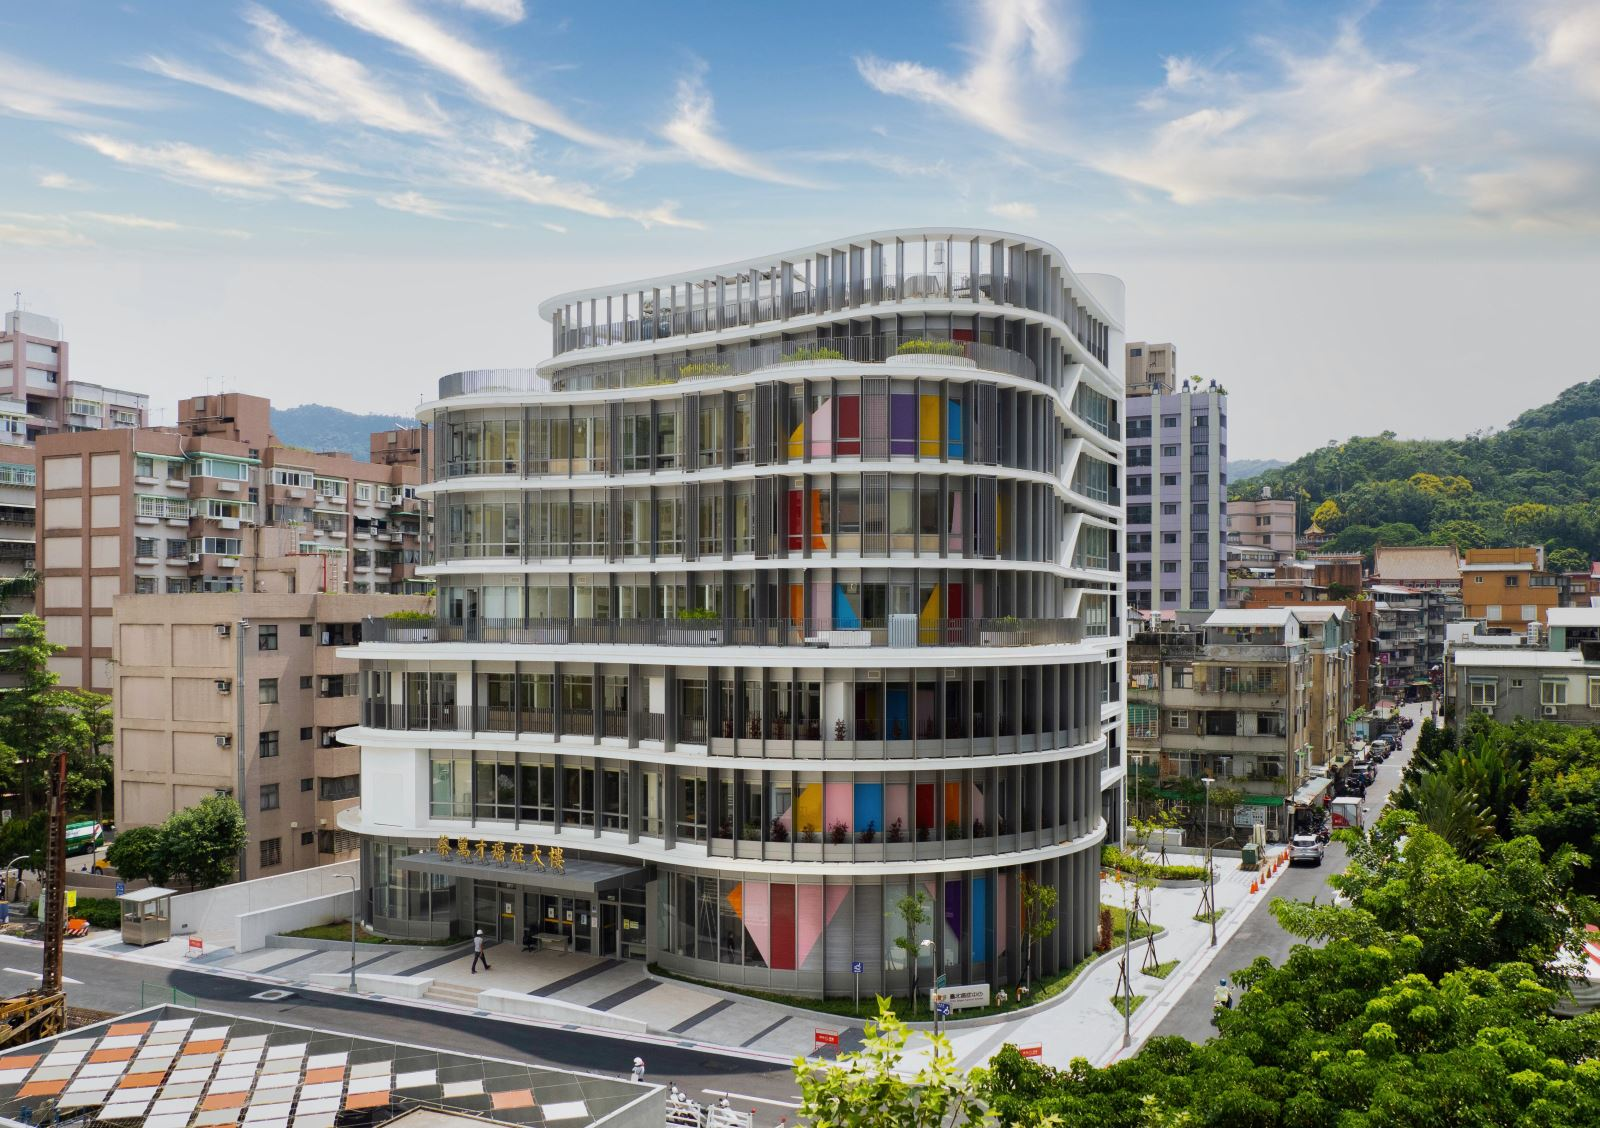
\includegraphics[width=0.75\linewidth]{295B6224-4030-47C6-9742-E3874C20445E.jpeg}
    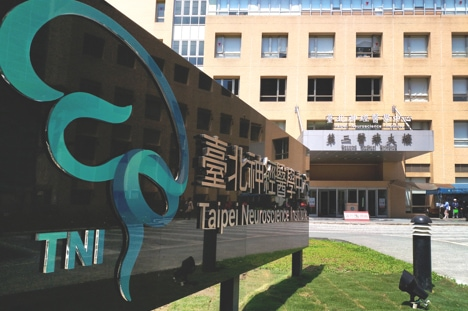
\includegraphics[width=0.75\linewidth]{6C597AEE-0ADA-4AC1-BA50-C500B9B911E0.jpeg}
    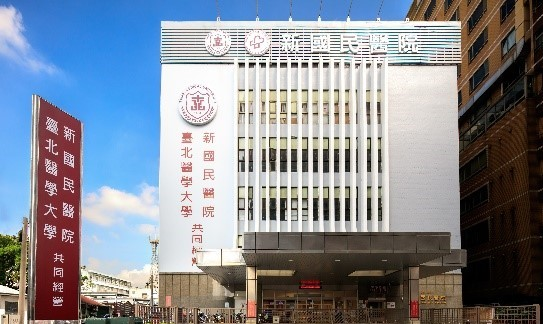
\includegraphics[width=0.75\linewidth]{17E0CB16-55CA-4F23-9A3A-F70CAE5FE133.jpeg}
\end{tikzfigure}
\end{minipage}


%%%

\block{Welcome to Taipei}{%
\begin{minipage}{0.3\linewidth}
  \centering
    \begin{tikzfigure}[Biomedical research]
    
\includegraphics[width=0.6\linewidth]{qrcode.jpeg}
    %TMU_QR_sholar.png}
%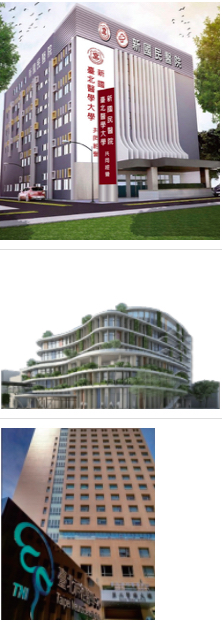
\includegraphics[width=0.5\linewidth]{TMU456.jpg}
    \end{tikzfigure}
\end{minipage}\hfill
\begin{minipage}{0.3\linewidth}
  \centering
\begin{tikzfigure}[Endoscopic simulation]
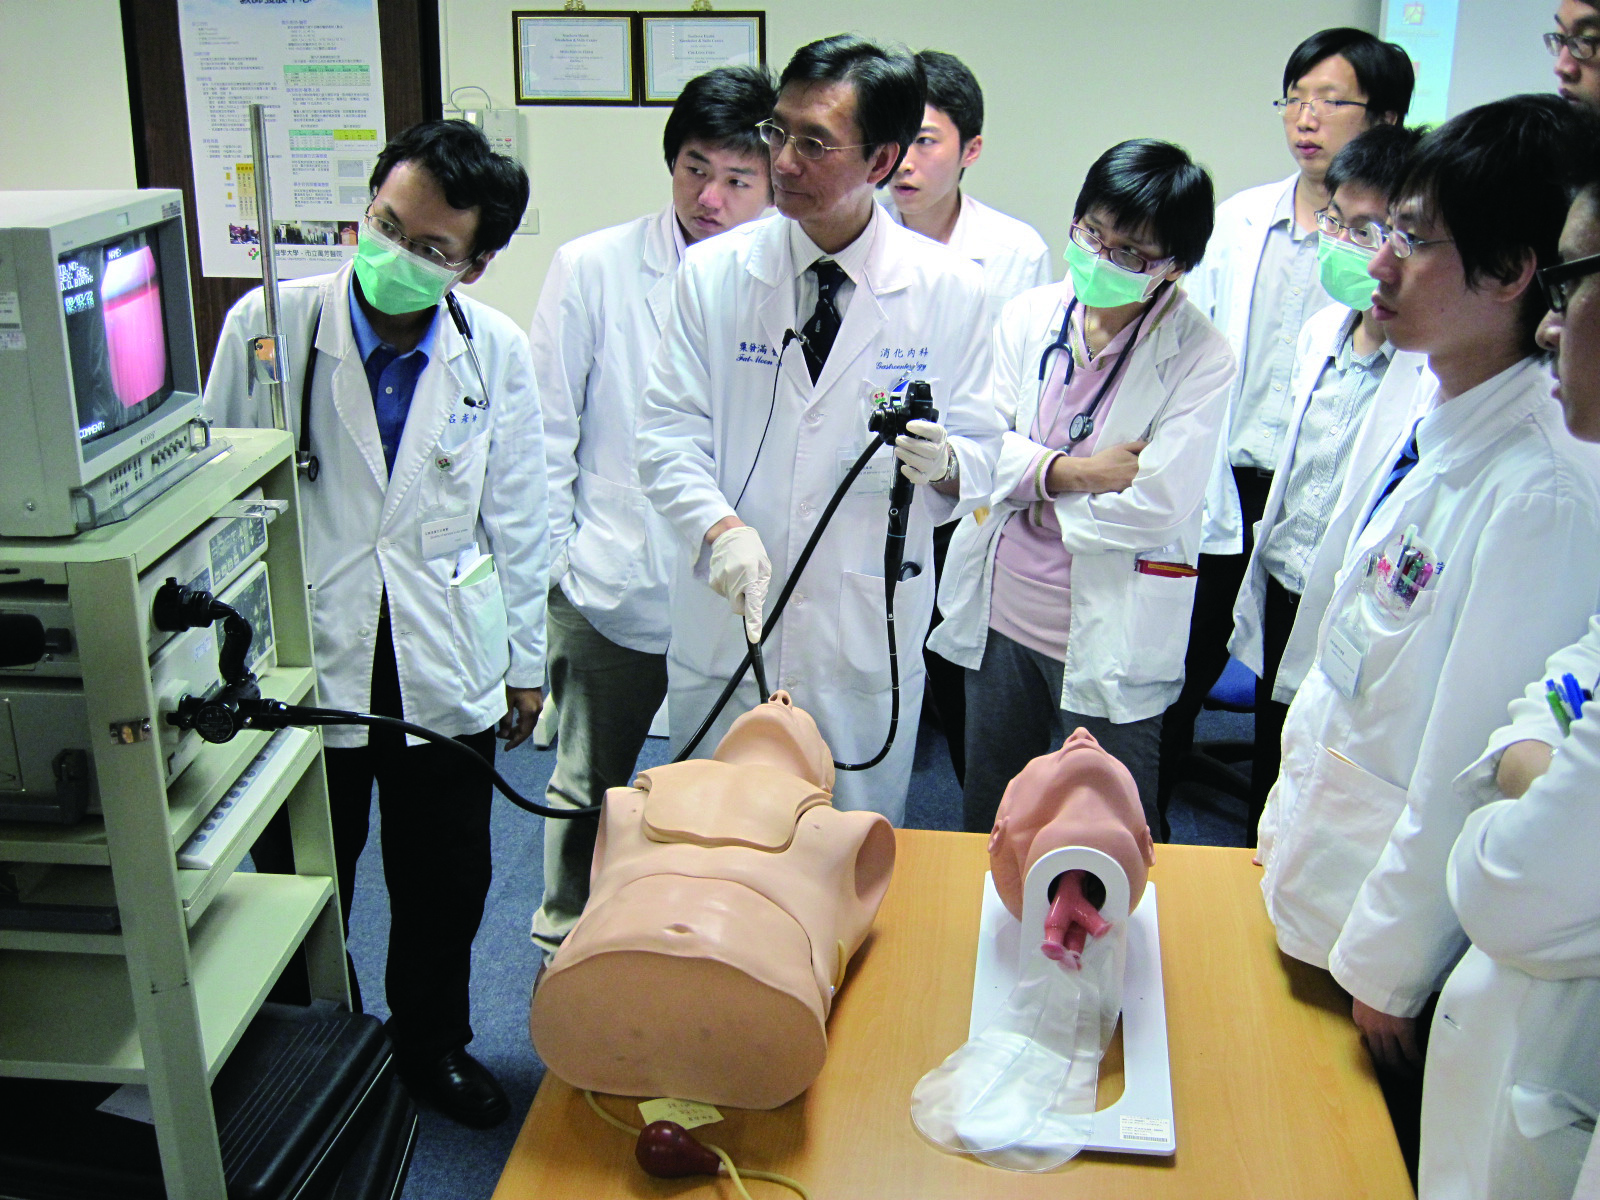
\includegraphics[width=0.7\linewidth]{2萬芳醫院中英文簡介照片.jpg}
\end{tikzfigure}  
\end{minipage}\hfill
\begin{minipage}{0.3\linewidth}
  \centering
\begin{tikzfigure}[Medical travel]

\includegraphics[width=0.65\linewidth]{qrcode.66164813.jpg}
\end{tikzfigure}
\end{minipage}

%(* photos courtesy of Studyportals B.V., and Public Relation \& Publishing Section, TMU Secretariat)
} % end of block
